%----------------------------------------------------------------------------
\chapter{\FurtherDevelopment}
%----------------------------------------------------------------------------

%----------------------------------------------------------------------------
\section{Üzemeltetési tapasztalatok}
%----------------------------------------------------------------------------

A megvalósított rendszer üzemeltetése a tervezett módon történt. A rendszer
tökéletesen megfelelt a kitett elvárásoknak, és üzemeltetése során nem
tapasztaltunk semmilyen rendellenességet. A teljesítménye és megbízhatósága is megfelelőnek bizonyult, nem 
voltak csomagvesztések a hálózaton, egyetlen egyszer sem kellett a másodlagos redundáns hálózatra
váltani, nem fordultak elő kiugró késések, minden eszköz bőven a beállított buffer méretben belül maradt.
Minden komponens megfelelően végezte a rá bízott feladatot, és a rendszer
stabilan kihagyás nélkül működött a teljes üzemidő alatt. 

%----------------------------------------------------------------------------
\section{Továbbfejlesztési lehetőségek}
%----------------------------------------------------------------------------


%----------------------------------------------------------------------------
\subsection{További eszközök integrálása}
%----------------------------------------------------------------------------

A Dante networking keresztrendszer lehetővé teszi a rendszer folyamatos bővítését a
hálózati limitációk megfelelő kezelésével. A rendszer bővítésekor figyelembe kell venni a
még rendelkezésre álló, a sávszélességet és a késleltetést mértékét. Amennyiben
tarjuk magunkat ezekhez a paraméterekhez, a rendszer bővítése nem okozhat problémát,
és megfelelő overhead mellett elméletileg a teljes hálózatot is szaturálhatjuk mindenféle probléma nélkül.
A Martin Audio Wavefront sorozatú hangfalak skálázható felbontása lehetővé teszi, hogy
a rendszer bővítésekor a már meglévő hangrendszerünket több végfokkal hajtva tovább
növeljük a rendszer teljesítőképességét. A korábbiakban már említett felbontás növelés
javítja a rendszer hangminőségét, frekvenciafelbontását és az adott területen való
pontosabb hangeloszlást. Ebből kifolyólag nagy fejlesztés lehet a jövőben a rendszer egy ládás
felbontásra való kibővítése. Ez azt jelenti, hogy az összes Line Array egységet külön-külön
végfok csatornával hajtjuk meg.
További fejlesztés a rendszerben a LineArray hangfalak számának növelése megfelelő számú végfok egységgel,
amely tovább növeli a rendszer teljesítményét és a maximálisan lefedhető területet.

%----------------------------------------------------------------------------
\subsubsection{Shure Axient Digital rendszer} % A jel egyből a Dante hálózaton keresztül érkezik a keverőbe nincs A/D konverzió
%----------------------------------------------------------------------------

%----------------------------------------------------------------------------
\subsubsection{TASCAM multitrack recorder} %TASCAM – DA-6400
%----------------------------------------------------------------------------

%----------------------------------------------------------------------------
\subsubsection{Allen \& Heath ME Personal Mixing System} % Előadóknak egyéni keverési lehetőség
%----------------------------------------------------------------------------
% ME-U + M-DANTE kártya + ME-500



%----------------------------------------------------------------------------
\begin
    {figure}[H]
    \centering
    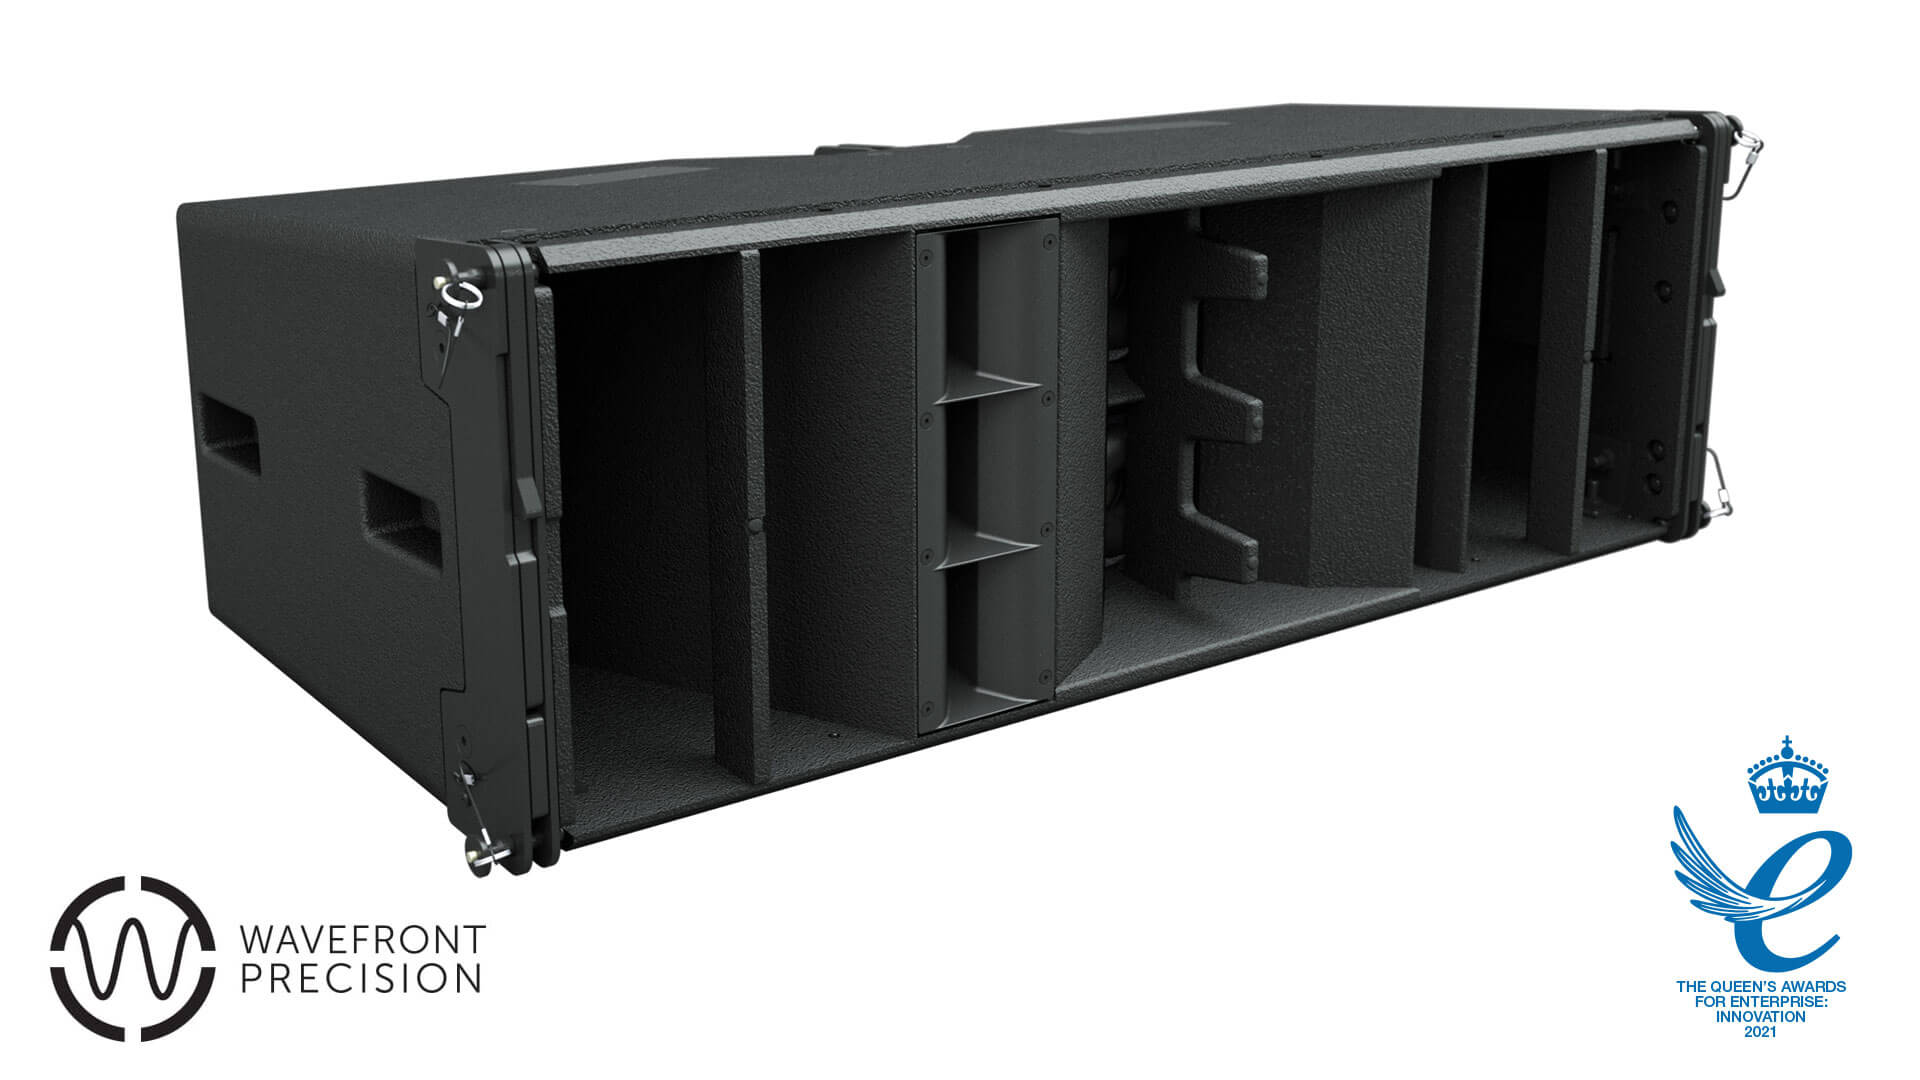
\includegraphics[width=80mm, keepaspectratio]{figures/wpl_front_view.jpg}
    \caption{Martin Audio WPL LineArray modul}
    \label{fig:martin_audio_wpl}
\end{figure}
%----------------------------------------------------------------------------

Amennyiben egy sokkal nagyobb rendezvényről van szó, és a jelenlegi rendszerünk már nem
tudná lefedni a területet, akkor a rendszer bővítése mellett egy nagyobb szériás LineArray
rendszer beszerzése is szükséges lehet. A Martin Audio WPL sorozatú ládái a jelenleg
elérhető legnagyobb terméke a Wavefront Precision sorozatban. 
Ebben az esetben a fő rendszert a WPL képviselné és WPC lenne az in-out fill rendszer.
A WPM szériás ládák pedig delayként szolgálnának a terület hátsó részén.
Viszont az említett teljes rendszerbővítésnek jelentős költségei vannak, így a rendszer
bővítése előtt alaposan mérlegelni kell, hogy valóban szükséges-e a rendszer bővítése,
megtérül-e a befektetés hosszabb távon.

Ha a megrendelő igényli, akkor a rendszerhez különböző rögzítő eszközöket is beszerezhetünk.
Lehetőségünk van megfelelő rögzítővel akár sávonként felvételt készíteni a koncertekről,
amelyeket később visszahallgathatunk, vagy akár további feldolgozásra is továbbíthatunk.
Emellett persze érdemes az élőben készült fő mix-et is rögzíteni a biztonság kedvéért.

Ha a jövőben több vezeték nélküli mikrofonra is szükségünk lenne, akkor a rendszer bővítése
során érdemes lehet nagyobb vezeték nélküli mikrofon rendszert is beszerezni. A jelenlegi
rendszert a Shure Axient Digital sorozatú rendszerekkel lehetne bővíteni, amelyek
kiváló minőségű vezeték nélküli mikrofonokat kínálnak, és a Dante hálózaton keresztül
könnyen integrálhatóak a már meglévő rendszerbe. Ez a rendszer is jelentős költségekkel
jár, így a bővítés előtt alaposan mérlegelni kell, hogy valóban szükséges-e a rendszer bővítése.



%----------------------------------------------------------------------------
\subsection{Bővítés nagyobb interfészre}
%----------------------------------------------------------------------------

Tegyük fel, hogy egy szimfonikus zenekar koncertjét szeretnénk hangosítani, ahol a zenekar
tagjainak száma meghaladja a 64 főt és mindenki dedikált mikrofonnal rendelkezik. Ebben az
esetben a 64x64-es Dante interfész már nem elegendő, mivel a zenekar tagjainak száma
meghaladja a csatornaszámot. Ebben az esetben a rendszer bővítésére van szükség.
Így az Allen \& Heath SQ sorozatú keverőpultjai már nem elegendőek, mivel ezekbe a keverőkbe ez az interfész a maximális.
Ebben az esetben egy nagyobb csatornaszámú keverőpultot kell választanunk, amelyek közül a
az Avantis és a dLive sorozatú keverők jöhetnek szóba. Ezek a keverők már kaphatóak
128x128-as Dante interfésszel is, így megnövelve a csatornaszámot. Azonban ezek a keverők
jelentősen magasabb árkategóriába tartoznak, mint az SQ sorozatú keverők, így a bővítés
költsége is nagyobb lesz. A keverőpultok fejlesztése mellett szükséges további
stageboxokat is beszerezni az igényelt csatornaszám eléréséhez.

%----------------------------------------------------------------------------
\begin
    {figure}[H]
    \centering
    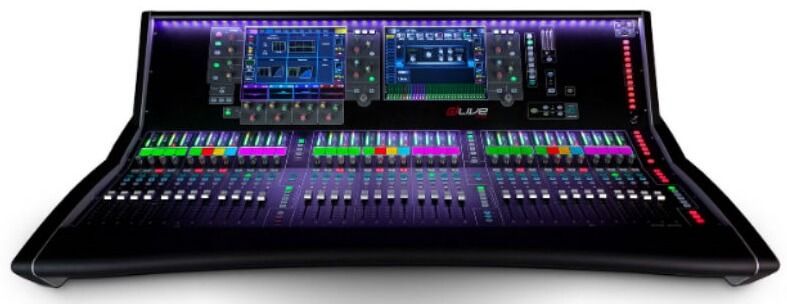
\includegraphics[width=80mm, keepaspectratio]{figures/dlive-s7000.jpg}
    \caption{Allen \& Heath dLive S7000 keverőpult}
    \label{fig:dLive_S7000}
\end{figure}
%----------------------------------------------------------------------------